\section{Leitungen}

\textbf{Aufgabe:}
\begin{itemize}
    \item  Energieübertragung und -verteilung\\
\end{itemize}

\textbf{Wichtigsten Leitungsarten:}
\begin{itemize}
    \item Freileitung
    \item Kabelleitung
    \item \textbf{Freileitungen} in praktisch allen Spannungsebenen von der Niederspannung bis zur Höchstspannung.
    \item \textbf{Kabelleitungen} mehr in den unteren Spannungsebenen.
\end{itemize}


\subsection{Freileitungen}

\begin{itemize}
    \item \textbf{Material:}
    \begin{itemize}
        \item Al-Seile (99{,}5\% Al), Aldrey-Seile (> 98{,}5\% Al, Mg, Si, Fe) und Al-Stahl-Seile\\ 
        (Verhältnis Alu:Stahl typ. 6:1, z.\,B. 240/40 mm\textsuperscript{2}), Kupfer ist bei neuen Leitungen immer seltener
        \item Aluminium-Drähten $\Rightarrow$ eine gute elektrische Leitfähigkeit
        \item Stahlkern $\Rightarrow$ mechanische Festigkeit
        \item Aluminium hat gegenüber Kupfer einen deutlichen Preisvorteil
    \end{itemize}

    \item Ab 220\,kV $\Rightarrow$ Bündelleiter $\Rightarrow$ Sie führen also zur 
    \textbf{Verminderung des Wellenwiderstandes} und damit 
    \textbf{zur Erhöhung der übertragbaren Leistung.}

    \item \textbf{Hochtemperaturleiter:}
    \begin{itemize}
        \item normale Leiterseile $T_{\text{max}} = 80\,^{\circ}\mathrm{C}$
        \item Hochtemperaturseilen $T_{\text{max}} = 210\,^{\circ}\mathrm{C}$
        \item \textbf{Steigerung der Übertragungskapazität um bis zu 50 Prozent}
    \end{itemize}
\end{itemize}


\subsection{Masten}

\textbf{Funktionen:}
\begin{itemize}
    \item \textbf{Tragmast:} Tragwerke für die Aufhängung der Leiter einer Freileitung
    \item \textbf{Abspannmasten:} An Winkelpunkten nehmen sie die Zugkräfte der Leiterseile auf.
    \item \textbf{Verdrillmast:} alle Aussenleiter eines Stromkreises auf dem Mast tauschen ihre Plätze\\
    (verbessertes Übertragungsverhalten).
\end{itemize}

\vspace{1em}
\textbf{Materialien:}
\begin{itemize}
    \item Stahl-Gittermast
    \item Betonmast
    \item Stahlrohrmast
    \item Holzmast
\end{itemize}


\subsection{Unterscheidungsmerkmale Freileitungen}

\textbf{Die wichtigsten Unterscheidungsmerkmale:}

\begin{itemize}
    \item Anzahl Phasen
    \item Länge der Isolatorenketten (Je höher die Spannung, umso länger sind die Isolatorenketten)
    \item Abstand der Phasen und Höhe der Masten
\end{itemize}

\begin{minipage}[c]{0.48\columnwidth}
    \begin{center}
        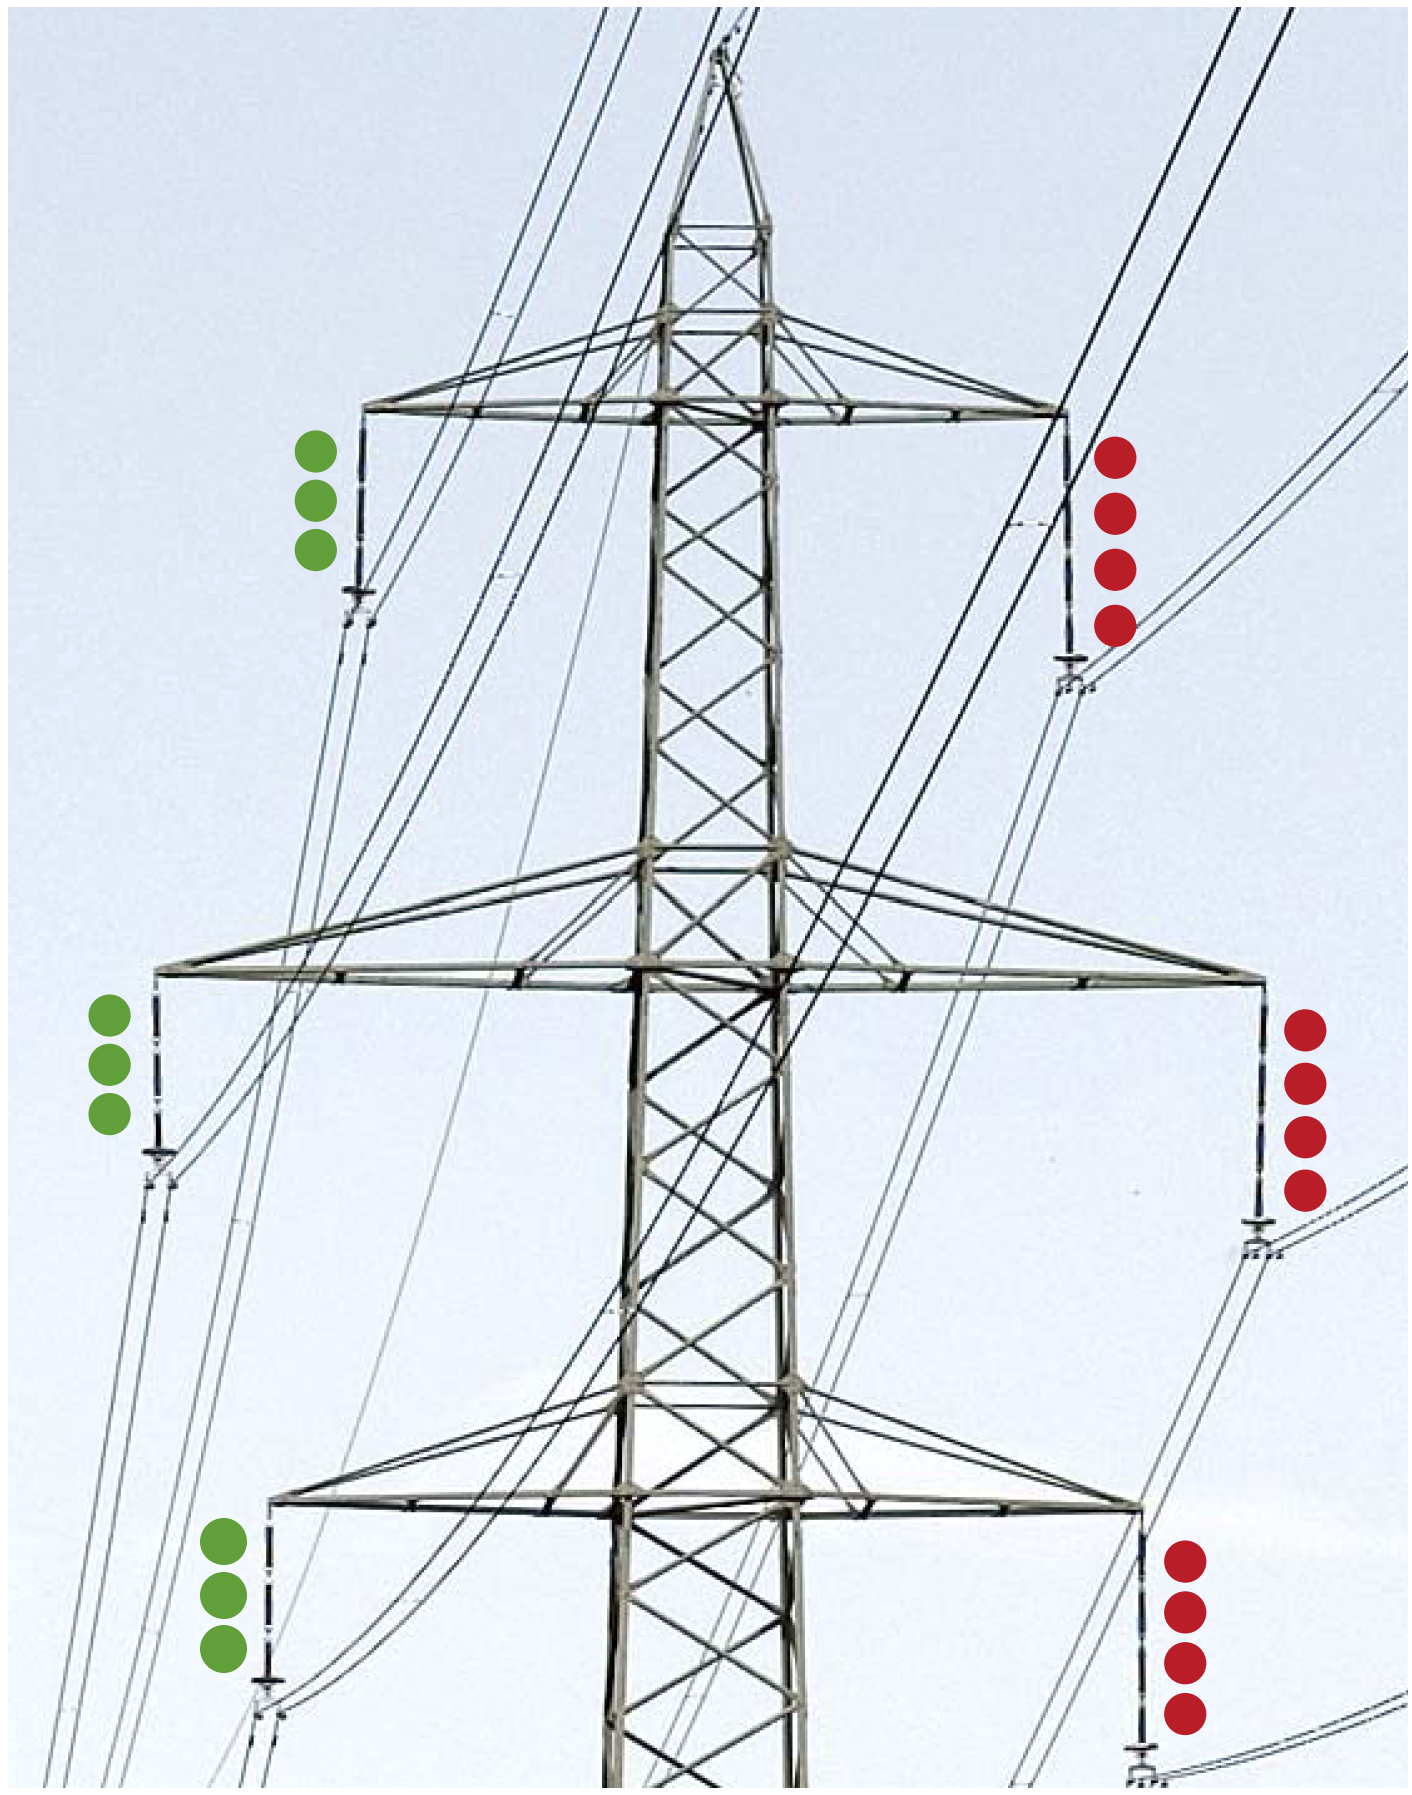
\includegraphics[width=0.9\textwidth, align=c]{images/Freileitungen_1.png}
    \end{center}
\end{minipage}
\hfill
\begin{minipage}[c]{0.48\columnwidth}
    \begin{center}
        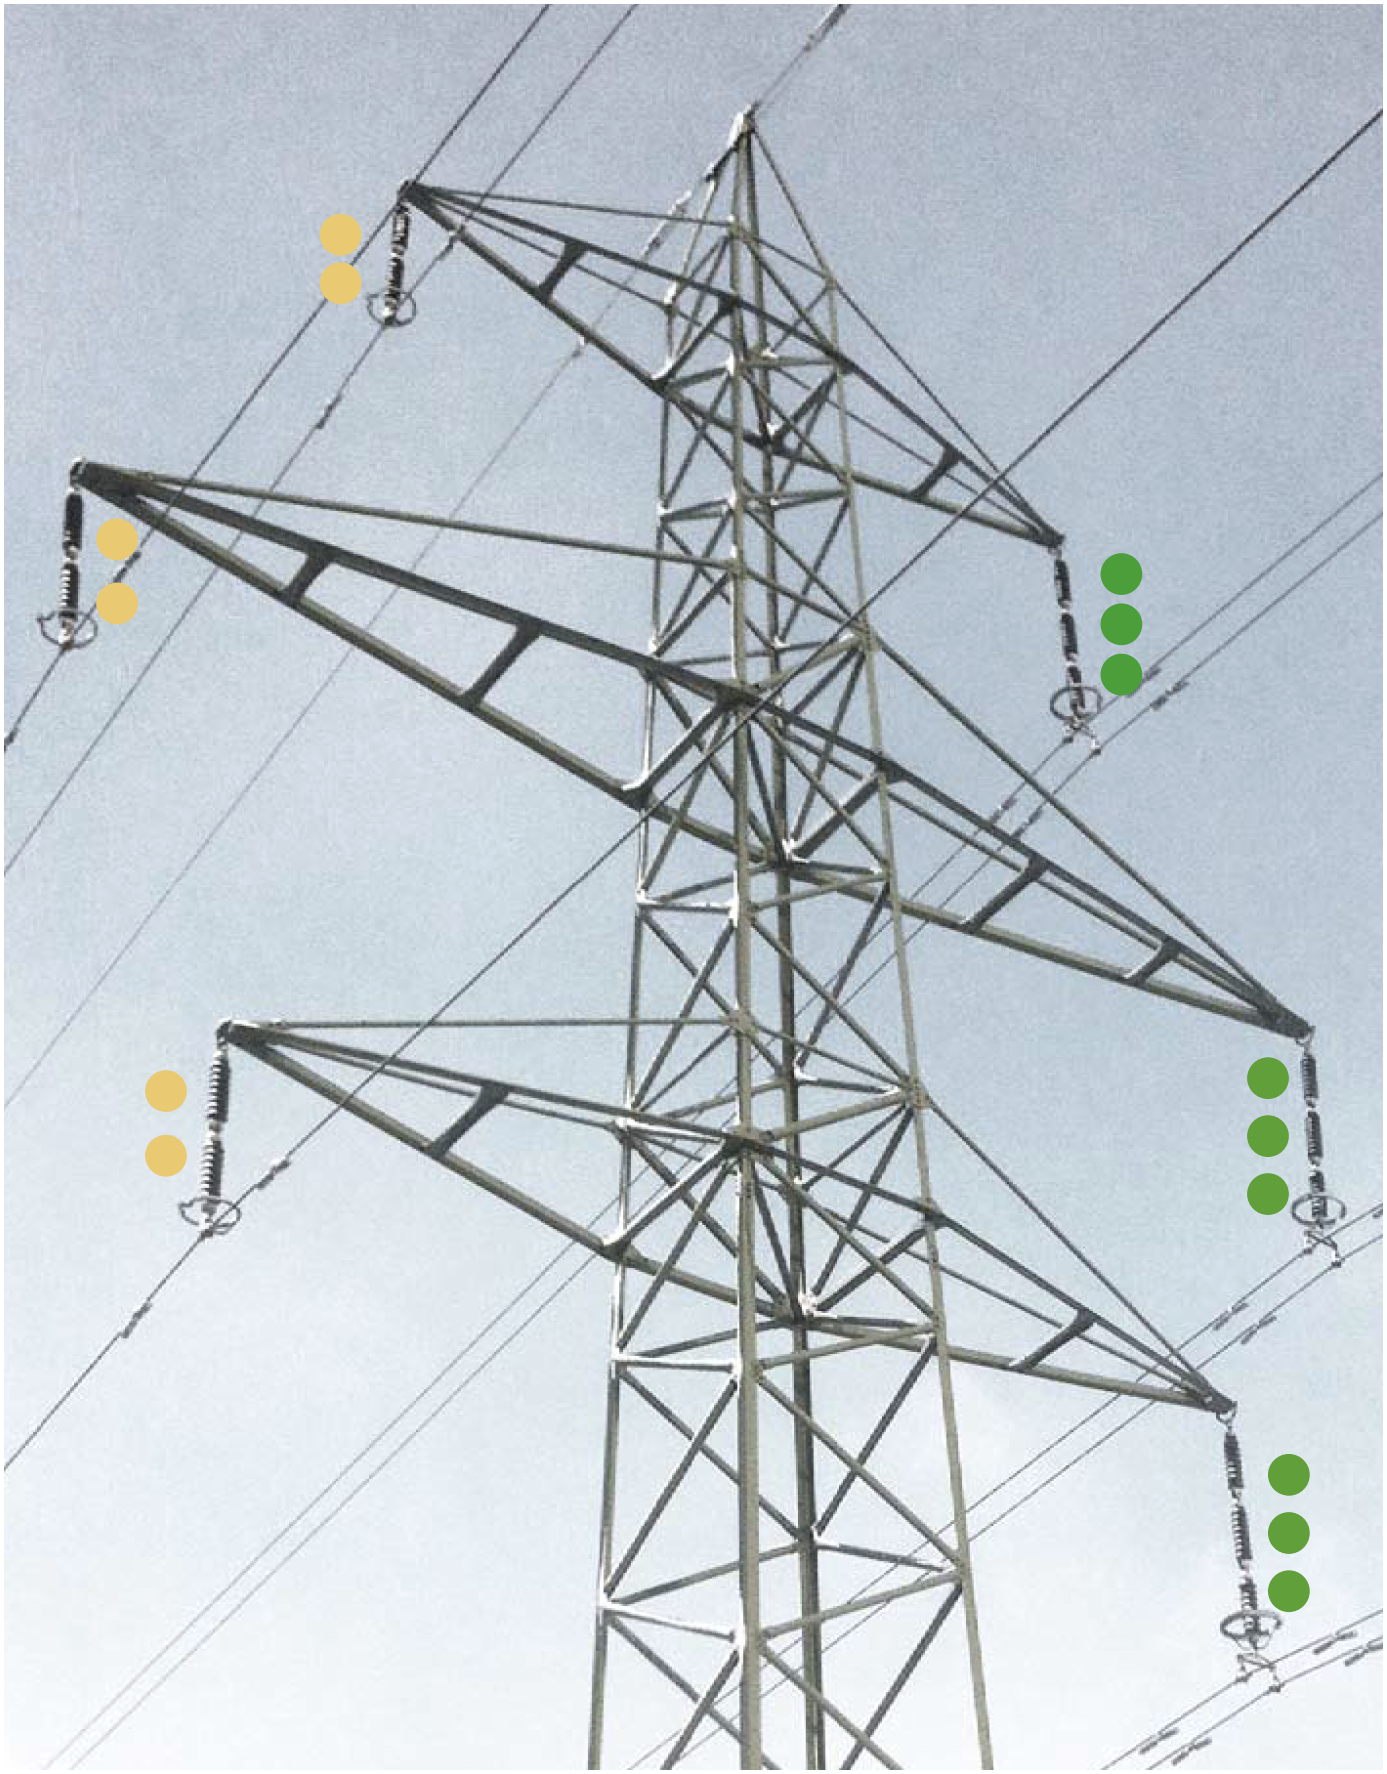
\includegraphics[width=0.9\textwidth, align=c]{images/Freileitungen_2.png}
    \end{center}
\end{minipage}

\subsection{Mastenformen}

\begin{minipage}[c]{0.4\columnwidth}
    \subsubsection{Donaumast}
\end{minipage}
\hfill
\begin{minipage}[c]{0.56\columnwidth}
    \subsubsection{Einebenenmast}
\end{minipage}

\begin{minipage}[c]{0.4\columnwidth}
    Zwei Drehstromkreise bei denen die Leiter jeweils im Dreieck angeordnet sind
\end{minipage}
\hfill
\begin{minipage}[c]{0.56\columnwidth}
    Niedrigen Bauhöhe und eine grössere Trassenbreite
\end{minipage}

\begin{minipage}[c]{0.4\columnwidth}
    \begin{center}
        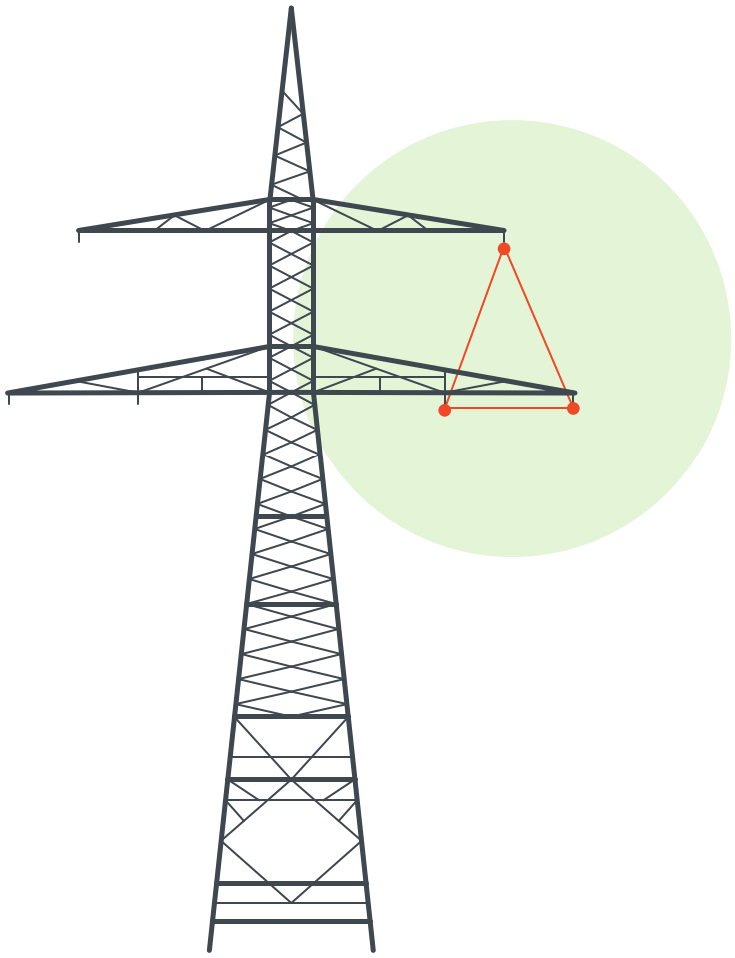
\includegraphics[height=5cm, align=c]{images/Mastenformen_1.png}
    \end{center}
\end{minipage}
\hfill
\begin{minipage}[c]{0.56\columnwidth}
    \begin{center}
        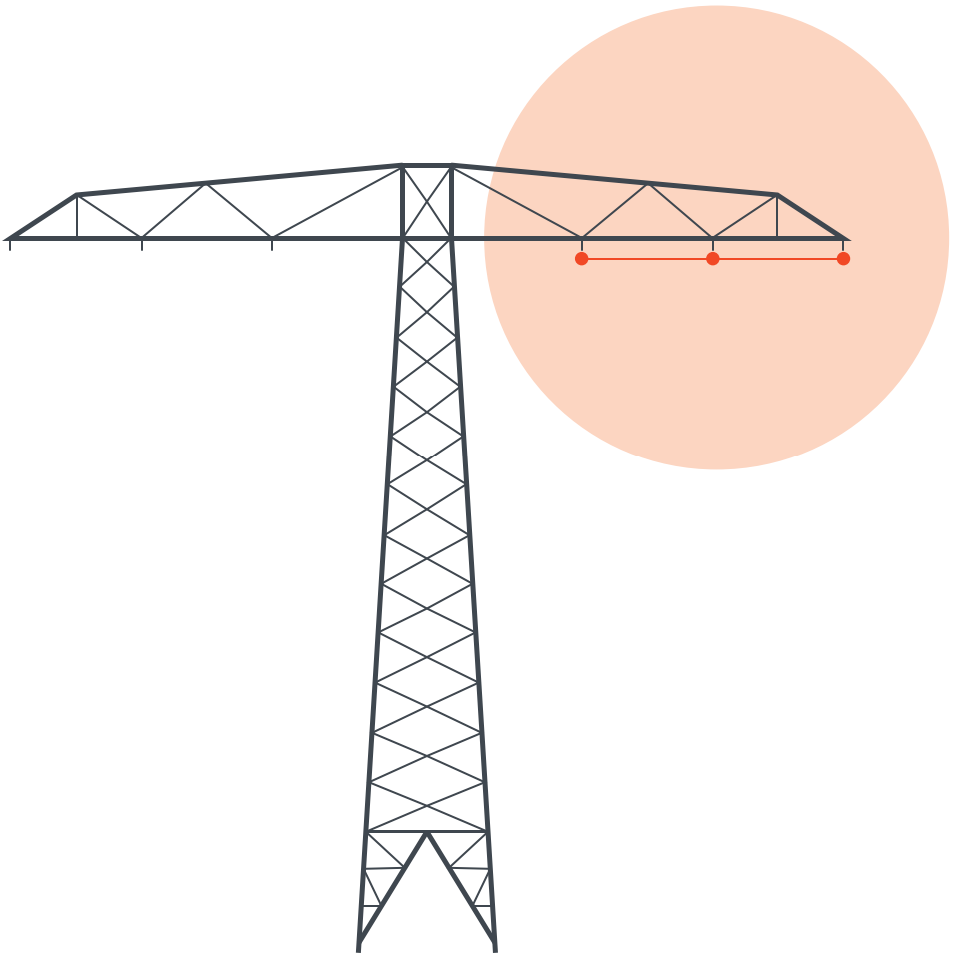
\includegraphics[height=5cm, align=c]{images/Mastenformen_2.png}
    \end{center}
\end{minipage}

\begin{minipage}[c]{0.5\columnwidth}
    \subsubsection{Tonnenmast}
    Eine geringe Trassenbreite, sind aber höher als vergleichbare Donaumasten

    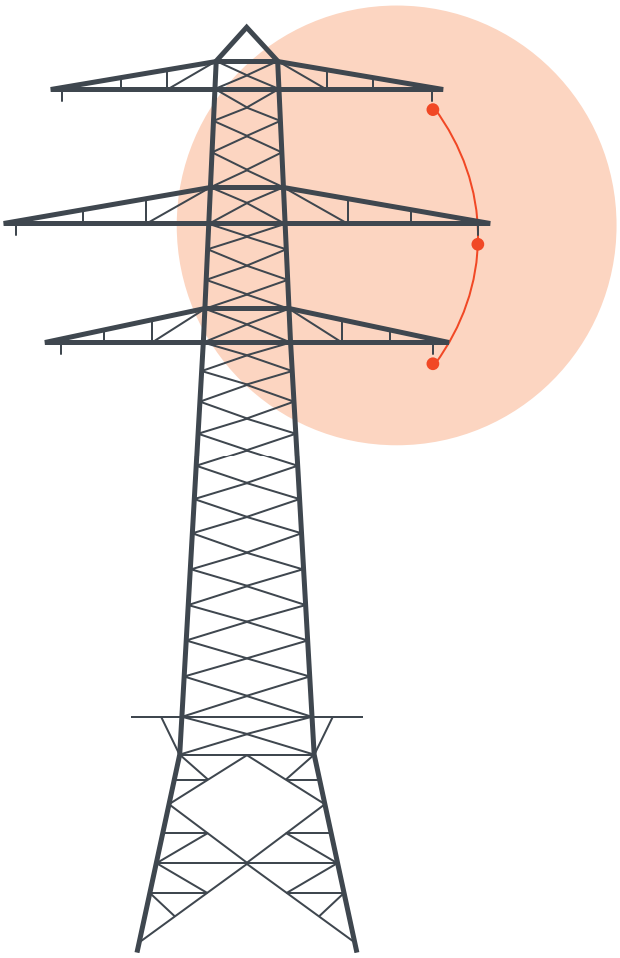
\includegraphics[height=5cm, align=c]{images/Mastenformen_3.png}    
\end{minipage}


\subsection{Freileitungen: Vor- und Nachteile}

\textbf{Pro:}
\begin{itemize}
    \item günstige Investitionskosten
    \item bessere Zugänglichkeit bei Reparaturen $\Rightarrow$ kürzere Wiederinbetriebnahmezeiten
\end{itemize}
\vspace{1em}
\textbf{Contra:}
\begin{itemize}
    \item atmosphärischen Einwirkungen ausgesetzt
    \item Akzeptanzprobleme
\end{itemize}


\section{Kabelleitungen}

\subsubsection{Material}

\begin{tabular}{>{\bfseries}l l}
    Leiter: & Kupfer oder Aluminium \\
    Isolierung: & öl-imprägniertes Papier oder Kunststoffe wie Polyäthylen (PE), \\
                & vernetztes Polyäthylen (VPE) sowie Polyvinylchlorid (PVC) \\
    Schutzmantel: & Metall \\
\end{tabular}


\subsection{Aufbau Allgemein}


\subsection{Aufbau}

\textbf{Gürtelkabel:}\\
Nichtradiales elektrisches Feld, Verwendung im Nieder- und Mittelspannungsbereich

\textbf{Dreimantel-Kabel:}\\
Radiales elektrisches Feld, Verwendung im Nieder- und Mittelspannungsbereich

\textbf{Einleiterkabel:}\\
Radiales elektrisches Feld, Verwendung im oberen Mittelspannungs- und im Hochpannungsbereich





\subsubsection{Kabel: Vor- und Nachteile}

\textbf{Pro:}
\begin{itemize}
    \item geschützt vor atmosphärischen Einwirkungen $\Rightarrow$ kleinere Ausfallsrate
    \item bessere Akzeptanz
\end{itemize}

\vspace{1em}
\textbf{Contra:}
\begin{itemize}
    \item schwierigere Zugänglichkeit bei Reparaturen $\Rightarrow$ längere Wiederinbetriebnahmezeiten
    \item im Hochspannungsbereich teurer (wirtschaftlich nur für kurze Strecken)
\end{itemize}


\subsection{Erdverkabelung in der Schweiz}

\textbf{Erdverkabelung pro Netzebene in der Schweiz}\\
\begin{tabular}{>{\bfseries}l r}
    Netzebene 1 & 8 km \\
    Netzebene 3 & 1'893 km \\
    Netzebene 5 & 30'607 km \\
    Netzebene 7 & 72'852 km \\
\end{tabular}



















